% should be sigplan instead of acmsmall?
\documentclass[acmsmall]{acmart}
%%
%% \BibTeX command to typeset BibTeX logo in the docs
\AtBeginDocument{%
  \providecommand\BibTeX{{%
    Bib\TeX}}}

\usepackage{tikz}
\usepackage{mathpartir}
%\usepackage[colorlinks=true, linkcolor=blue]{hyperref}
\usepackage[capitalise]{cleveref}
\usepackage{hyperref}
% this doesn't seem to be working...
\hypersetup{
    colorlinks=true,
    linkcolor=blue,
    urlcolor=cyan,
    }

%% Commands
\newcommand{\rec}{\mathsf{rec}}
\newcommand{\VType}{\mathbf{VType}}
\newcommand{\CType}{\mathbf{CType}}
\newcommand{\Prop}{\mathbf{Prop}}

\newcommand{\isVType}{\textrm{ VType}}
\newcommand{\isCType}{\textrm{ CType}}
\newcommand{\isProp}{\textrm{ Prop}}
\newcommand{\isCtx}{\textrm{ Ctx}}

\newcommand{\ctxjdg}[1]{#1 \isCtx}
\newcommand{\vtypejdg}[2]{#1 \vdash #2 \isVType}
\newcommand{\ctypejdg}[2]{#1 \vdash #2 \isCType}
\newcommand{\vtrmjdg}[3]{#1 \vdash #2 : #3}
\newcommand{\ctrmjdg}[3]{#1 \vdash #2 : #3}

\newcommand{\den}[1]{\llbracket #1\rrbracket}
\newcommand{\denLctx}[1]{\den{#1}^L_{ctx}}
\newcommand{\denLty}[1]{\den{#1}^L_{ty}}
\newcommand{\denLtm}[1]{\den{#1}^L_{tm}}

\newcommand{\obliv}[2]{\mathcal{O}_{#1}({#2})}
\newcommand{\wrap}[2]{\mathcal{W}_{#1}({#2})}


\newcommand{\bool}{\mathbb{B}}
\newcommand{\true}{\mathtt{true}}
\newcommand{\false}{\mathtt{false}}
\newcommand{\nat}{\mathbb{N}}

\newcommand{\eric}[1]{\textcolor{red}{ <eric-#1> }}

%% Rights management information.  This information is sent to you
%% when you complete the rights form.  These commands have SAMPLE
%% values in them; it is your responsibility as an author to replace
%% the commands and values with those provided to you when you
%% complete the rights form.
\setcopyright{acmlicensed}
\copyrightyear{2018}
\acmYear{2018}
\acmDOI{XXXXXXX.XXXXXXX}
%% These commands are for a PROCEEDINGS abstract or paper.
\acmConference[Conference acronym 'XX]{Make sure to enter the correct
  conference title from your rights confirmation email}{June 03--05,
  2018}{Woodstock, NY}
%%
%%  Uncomment \acmBooktitle if the title of the proceedings is different
%%  from ``Proceedings of ...''!
%%
%%\acmBooktitle{Woodstock '18: ACM Symposium on Neural Gaze Detection,
%%  June 03--05, 2018, Woodstock, NY}
\acmISBN{978-1-4503-XXXX-X/2018/06}


%% Submission ID.
%% Use this when submitting an article to a sponsored event. You'll
%% receive a unique submission ID from the organizers
%% of the event, and this ID should be used as the parameter to this command.
%%\acmSubmissionID{123-A56-BU3}


\begin{document}

%%
%% The "title" command has an optional parameter,
%% allowing the author to define a "short title" to be used in page headers.
\title{Fresh Parametricity}


\author{Eric Bond}
\email{bonderic@umich.edu}
\affiliation{%
  \institution{University of Michigan}
  \city{Ann Arbor}
  \country{USA}
}

\author{Max New}
\affiliation{%
  \institution{University of Michigan}
  \city{Ann Arbor}
  \country{USA}
}

%%\renewcommand{\shortauthors}{Trovato et al.}


\begin{abstract}
  ABSTRACT 
  $\Prop$
\end{abstract}

%%
%% The code below is generated by the tool at http://dl.acm.org/ccs.cfm.
%% Please copy and paste the code instead of the example below.
%%
\begin{CCSXML}
<ccs2012>
 <concept>
  <concept_id>00000000.0000000.0000000</concept_id>
  <concept_desc>Do Not Use This Code, Generate the Correct Terms for Your Paper</concept_desc>
  <concept_significance>500</concept_significance>
 </concept>
 <concept>
  <concept_id>00000000.00000000.00000000</concept_id>
  <concept_desc>Do Not Use This Code, Generate the Correct Terms for Your Paper</concept_desc>
  <concept_significance>300</concept_significance>
 </concept>
 <concept>
  <concept_id>00000000.00000000.00000000</concept_id>
  <concept_desc>Do Not Use This Code, Generate the Correct Terms for Your Paper</concept_desc>
  <concept_significance>100</concept_significance>
 </concept>
 <concept>
  <concept_id>00000000.00000000.00000000</concept_id>
  <concept_desc>Do Not Use This Code, Generate the Correct Terms for Your Paper</concept_desc>
  <concept_significance>100</concept_significance>
 </concept>
</ccs2012>
\end{CCSXML}

\ccsdesc[500]{Do Not Use This Code~Generate the Correct Terms for Your Paper}
\ccsdesc[300]{Do Not Use This Code~Generate the Correct Terms for Your Paper}
\ccsdesc{Do Not Use This Code~Generate the Correct Terms for Your Paper}
\ccsdesc[100]{Do Not Use This Code~Generate the Correct Terms for Your Paper}

%% Keywords. The author(s) should pick words that accurately describe
%% the work being presented. Separate the keywords with commas.
\keywords{Do, Not, Us, This, Code, Put, the, Correct, Terms, for,
  Your, Paper}


\received{20 February 2007}
\received[revised]{12 March 2009}
\received[accepted]{5 June 2009}


\maketitle

\section{Introduction}
\eric{no "type instantiations"}
\eric{fresh param instead of non-standard}
\subsection{Parametricity}
\eric{decide how you want to introduce parametrictiy, then work on flow}
Parametricity states \eric{wording}that any term of a universal or existential type must behave uniformly for any possible type instantiation.
Existential types can be used to encode abstract data types like Queues or Graphs. 
If we know our language enjoys parametric polymorphism, then we have a guarantee that any two instance of a Queue, as encoded by an existential type, are observationally equivalent.
Meaning, we can swap implementations of the Queue data type without changing the correctness of the overall program. (ignoring resource constraints, time/space)
Universal types in a parametrically polymorphic language allow for a sound implementation of church encoded data. 
Theorems for free
	\eric{
	Address this first, then provide examples?}

\subsection{Parametricity vs Intensional Type Analysis}
\eric{Dyn or ?}
While parametricity is a desirable property, it is hard to maintain with certain language features that use \textit{intensional type analysis} \cite{IntTypeAnalysis}. By Intensional type analysis, we mean the ability to inspect the run time representaiton of a type and dispatch based on the result. \eric{wording}An example of this behavior is the casting rules in a gradual typed language\cite{GradParam}.


\subsubsection{Gradual Typing}
Gradual typing allows programmers gradually migrate from \eric{dynamically/untyped} code to typed code by including a type $Dyn$ representing a dynamically checked term. 
The interface between dynamically typed code and statically typed code is handled by casting.
A value of any type $A$ can be up cast $\uparrow_A^?$ to the dynamic type.
Downcasting $\downarrow_A^?$from the dynamic type can introduce errors if the value stored in Dyn is not of the requested type.
Naively adding Dyn, up casting, and down casting to a parametrically polymorphic language breaks parametricity. 
Consider a polymorphic gradually typed language which can error.
$$t : \forall X. X \rightarrow \mathbb{B}:= (\Lambda X. \lambda (x : X). \downarrow_\mathbb{B}^?\uparrow_X^?(x))$$

\eric{$\mathbb{B}$ and Bool used here}
If we assume that $t$ behaved uniformly for all possible type instantiations, then $t$ should either error
or return a boolean that is not dependent on the argument of type $X$.
But this is not the case \eric{grammar}
when instantiated at type Bool, $t$ will return the given boolean value
$t[\mathbb{B}](b : \mathbb{B}) \leadsto^* b$ for any other type $A$ it will error
$t[A](x:A)\leadsto^* \Omega$
Therefore $t$ does not behave uniformly for all types. 
The issue here is that casting inspects the type tag used in the values stored in dyn, a case of intensional type analysis.

\subsection{Preserving Parametricity}
% many attempts to combine gradual typing and parametric polymorphism
% it has been demonstrated 

% Not just gradual typing.. intensional type analysis
The difficulties of combining parametric polymorphism and language features relying on type analysis are well known\cite{NonParam}\cite{GradParam}\cite{ToroGradParam}\cite{ForFreeForFree}.
Solutions that preserve parametricity usually involve a form of \textit{dynamic sealing} or generation of \textit{fresh type tags}. Reason being, the ability to inspect a type and dispatch based on the result is in direct conflict with the information hiding principle provided in a language with parametric polymorphism. By hiding information about the runtime representation of a type, we can restore the property that polymorphic types behave uniformly across all type instantiations.

While such techniques have demonstrated they can preserve the expected information hiding properties, they do so using a \textit{non-standard} formulation of parametricity. Specifically, the approach used by Niels\cite{NonParam} and New\cite{GradParam} invoke a \textit{Type-World} logical relation where the freshly allocated type variables/tags, $\alpha$, are associated with concrete types, $(A,A')$, and a relation, $R : Rel[A,A']$, on those types. This mapping, $\alpha \mapsto (A,A',R)$, of dynamically allocated type variable to concrete types and a relation are threaded through the logical relation via a Kripke world. A question remains, what is the relative strength of this non-standard formulation of parametricity compared to traditional definitions? In particular, does the \textit{type-world} formulation allows us to prove the \textit{free-theorems} and \textit{data-abstraction} properties we would should expect?\eric{introduce vocab? non-starndard param as type world param?}

\subsection{Failure of Full Abstraction}
This was partially answered in the affirmative by Nies et al\cite{NonParam}. The argument proceeds by introducing two languages: An effectful variant of CBV System F with a standard notion of parametricity, and System G, an extension of the former language with type casts and fresh type name allocation supporting a \textit{non-standard}, type world, formulation of parametricity.
To compare the languages, they provide a type preserving embedding, $\den{\_}$, from System F to System G. 

\begin{theorem}
  Preservation of Typing.
  $$\vdash_F V : A \implies \vdash_G \den{V} : \den{A}$$
\end{theorem}

The embedding, $\den{\vdash_F V:A} = \mathcal{W}_{A} \circ \den{\vdash_F V:A}^L$, is decomposed into a lifting, $\den{\_}^L$, and a type directed wrapping function $\mathcal{W}_A$. The lifting preserves syntactic equality of terms and types, so $V \equiv \den{V}^L$ and $A \equiv \den{A}^L$. The wrapping function is a deep $\eta$ expansion which strategically inserts fresh type allocation in the elimination forms of the universal and existential types. The purpose of the wrapping is to ensure that lifted polymorphic terms of System F are simultaneously safe from non-parametric uses and forced to behave parametrically in the presence of System G's type cast operation. More details can be found in \cref{sec:Wrap}. 

\begin{conjecture}
  \textbf{False}: Full Abstraction of $\den{\_}$
  $$\forall V_1,V_2. V_1\cong_F V_2 \implies \den{V_1} \cong_G \den{V_2}$$
\end{conjecture}

To demonstrate the relative strengths of the different notions of parametricity, they conjecture that the embeddings is \textit{fully-abstract}, preserving all the contextual equivalences of the original language. However, this conjecture was later disproven\cite{ParamVSUniv} \cite{TwoParamVSThreeUniv}. The counter example relies on the fact that the type $Univ := \exists Y.\forall X. (X\rightarrow Y)\times (Y \rightarrow X)$ must be \textit{degenerate} in effectful System F, but there are non-degenerate inhabitants of this type in System G. 

\subsection{Our Result}
\eric{rename section, more connective tissue}
Our aim is to demonstrate that, while the transformation does not preserve contextual equivalence, it preserves a weaker notion we call \textit{Logical Equivalence}. By Logical Equivalence, we mean to say that any results proven in a \textit{Parametricity Logic}\cite{APL}\cite{LAPL}\cite{PE} for effectful System F can be transfered to a parametricity logic backed by the non-standard, type-world, notion of parametricity.

%y constructing two parametricity logics. One for a language without fresh type generation, another for a language with fresh type generation. We then show that any two provably equal terms of the first logic are provable equal, under translation, in the second logic.
\eric{TODO: rename "Logic A" and "Logic B"(source/target?)}
\begin{theorem}
  Logical Equivalence:
  $$\Gamma \vdash_A M = N \implies \den{\Gamma} \vdash_B \den{M} = \den{N}$$
\end{theorem}

\eric{placeholder figure, refactor}
\begin{figure}[H]
  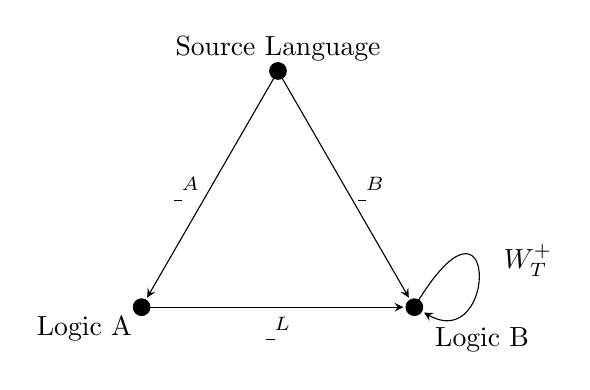
\begin{tikzpicture}[scale=2, ->, >=stealth]
    % Coordinates for triangle vertices
    \coordinate (A) at (0,1);            % Top: Source Language
    \coordinate (B) at (-0.866,-0.5);    % Bottom left: Logic A
    \coordinate (C) at (0.866,-0.5);     % Bottom right: Logic B
    % Draw dots and labels
    \filldraw (A) circle (1.5pt) node[above] {Source Language};
    \filldraw (B) circle (1.5pt) node[below left] {Logic A};
    \filldraw (C) circle (1.5pt) node[below right=4pt] {Logic B};
    % Arrows with labels and slight offset for arrowhead visibility
    \draw[->, shorten >=4pt] (A) -- (B) node[midway, left] {$\den{\_}^A$};
    \draw[->, shorten >=4pt] (A) -- (C) node[midway, right] {$\den{\_}^B$};
    \draw[->, shorten >=4pt] (B) -- (C) node[midway, below] {$\den{\_}^L$};
    % Self-loop on Logic B, label offset to avoid overlap
    \draw[->, shorten >=4pt] (C) .. controls (1.4,0.4) and (1.4,-0.8) .. (C)
  node[pos=0.5, right=6pt, yshift=4pt] {$W^+_T$};
  \end{tikzpicture}
\end{figure}

\subsection{Overview}

\eric{bullet format or paragraph?}
 To demonstrate the preservation of logical equivalence we first define an effectful CBV variant of System F in \cref{sec:SourceLang} for which we want our theorem to apply to. We then define the \textit{object languages} of our paremetricity logics in \cref{sec:ObjLang} which are effectful, CBPV \cite{CBPV} variants of System F. We then define the translations of the source language to each of these object languages \eric{cref}. The translations will largely follow the usual\cite{CBPV} CBV to CBPV translation, with a few exceptions, notably the parametricity preserving wrapping in \cref{sec:Wrap}. In \cref{sec:Logics}, we will introduce our parametricity logics\eric{cref} and the translation \eric{cref} between the logics.
 \eric{compositionality issues.. oblivious predicate..adequacy..example proof in Logic..discussion/relatedwork.. order TBD here.. come back to this}







\begin{comment}
\subsubsection{Gradual Typing with Fresh Quantification}

To illustrate this, we will consider a polymorphic Call-by-push-value \eric{cite} calculus with an extensible sum type denoted $OSum$ which we use to represent the dynamic type Dyn. In order to inject a value, $V:A$, into $OSum$, we need a $Case$ symbol associated with the type $A$. Case symbols are representative of the runtime type tags of the dynamic type and can be dynamically allocated by the expression $new_A : F(Case\;A)$. The introduction from of the extensible sum type, $inj_\sigma\;V : OSum$ uses a case symbol $\sigma : Case\;A$ to store a value $V:A$. The elimination form, $rec_{OSum}\;(inj_\sigma\;V),\sigma'\;\{x.\;M\;|\;N\}$, compares the case symbol $\sigma$ used to inject the value into $OSum$ to a given case symbol $\sigma'$. When the case symbols match, the value stored in $OSum$ is bound to $x$ in the continuation $M$. Otherwise, we proceed with the default case $N$. Assuming a preallocated set of case symbols $\sigma_\mathbb{B} : Case\;\mathbb{B},\sigma_\times : Case\;(OSum \times OSum),\sigma_\to : Case\;(OSum \to OSum),...$, we can encode the example above as:
$$t : \forall X.Case\;X \to X \to F\mathbb{B} := \Lambda X. \lambda \sigma_X.\lambda x.rec_{OSum}\;(inj_{\sigma_X}x),\sigma_\mathbb{B}\;\{x.\;ret\;x\;|\;\Omega\}$$
\\
\\
% preserve parametricity reasoning?
\end{comment}




\section{Languages}\label{sec:Languages}
\begin{itemize}
  \item section overview.
  \item why have a source language
  \item why CBPV
\end{itemize}
\subsection{Source Language}\label{sec:SourceLang}
\eric{remove existential for now}
\begin{itemize}
  \item why "jumbo" connective (not jumbo, just greater airity)
  \item why general recursion and error? (OSum can encode these)
\end{itemize}
\begin{figure}[H]
  \begin{mathpar}
    \footnotesize
    \inferrule{ }{\Gamma,X \vdash X \; Type}
    \and
    \inferrule{ }{\Gamma \vdash \mathbb{B} \; Type}
    \and
    \inferrule{ }{\Gamma \vdash \mathbb{N} \; Type}
    \and
    \inferrule{\Gamma \vdash A \; Type \\ \Gamma \vdash A' \; Type}
              {\Gamma \vdash A \times A' \; Type}
    \and
    \inferrule{\Gamma,X \vdash A \; Type}
              {\Gamma \vdash \exists X.A}
    \and
    \inferrule{\Gamma,\overrightarrow{X}_n \vdash A_i \; Type \;\;\forall i \in \{m\} \\
               \Gamma,\overrightarrow{X}_n \vdash A \; Type}
              {\Gamma \vdash \forall[\overrightarrow{X}_n].(\overrightarrow{A}_m)\rightarrow A \; Type}
  \end{mathpar}
  \caption{Source Language Type Formers}
  \label{fig:value-type-formers}
\end{figure}


\begin{figure}[H]
  \begin{mathpar}
    \footnotesize
    \inferrule{ }{\Gamma ,x : A \vdash x : A}

    % Bool
    \and
    \inferrule{ }{\Gamma \vdash true : \mathbb{B}}
    \and
    \inferrule{ }{\Gamma \vdash false : \mathbb{B}}
    \and
    \inferrule{\Gamma \vdash b : \mathbb{B} \\ \Gamma \vdash M : A \\ \Gamma \vdash N : A}
              {\Gamma \vdash rec_{\mathbb{B}} \;b \; \{M\;|\;N\} : A}

    % Nat
    \and
    \inferrule{ }{\Gamma \vdash z : \mathbb{N}}
    \and
    \inferrule{\Gamma \vdash n : \mathbb{N}}
              {\Gamma \vdash s\;n : \mathbb{N}}
    \and
    \inferrule{\Gamma \vdash n : \mathbb{N} \\ \Gamma \vdash M : A \\ \Gamma,x : \mathbb{N} \vdash N : A}
              {\Gamma \vdash rec_{\mathbb{N}} \;n \; \{M\;|\; x.\;N\} : A}

    % Jumbo Function
    \and
    \inferrule{\Gamma,\overrightarrow{X}_n\vdash A_i \;Type\;\; \forall i\in \{m\} \\
              \Gamma,\overrightarrow{X}_n\vdash A' \;Type \\
              \Gamma,\overrightarrow{X}_n,x_1 : A_1,\cdots,x_m : A_m \vdash M : A'}
              {\Gamma \vdash \Lambda[\overrightarrow{X}_n](x_1 : A_1,\cdots,x_m:A_m).M : \forall[\overrightarrow{X}_n].(\overrightarrow{A}_m)\rightarrow A'}

    \and
    \inferrule{\Gamma \vdash A_i\;Type \;\;\forall i\in \{n\} \\
              \Gamma \vdash M : \forall[\overrightarrow{X}_n].(\overrightarrow{A}_m) \rightarrow A' \\
              \Gamma \vdash N_i : B_i[\overrightarrow{A}/\overrightarrow{X}] \; \forall i \in \{m\}}
              {\Gamma\vdash M[\overrightarrow{A}_n](N_1 : B_1,\cdots N_m : B_m) : A'}

    % Exists
    \and
    \inferrule{\Gamma \vdash V : T[A/X]}
              {\Gamma \vdash pack\langle A,V \rangle : \exists X. T}
    \and
    \inferrule{\Gamma  \vdash W : \exists X.T \\ \Gamma,A,V:T[A/X] \vdash M : A'}
              {\Gamma \vdash unpack\langle A, V\rangle = W; M : A'}

    % Product
    \and
    \inferrule{\Gamma \vdash M : A \\ \Gamma \vdash N : A}
              {\Gamma \vdash (M,N) : A \times A}
    \and
    \inferrule{\Gamma \vdash M : A\times A' \\ \Gamma,x:A,y:A' \vdash N : A}
              {\Gamma \vdash rec_\times \; M \;\{x,y.\; N\} : A''}

    % Error
    \and
    \inferrule{ }{\Gamma \vdash \Omega_A : A}

    % Fixpoint
    \and
    \inferrule{\Gamma , x : A \vdash V : A'}
              {\Gamma \vdash \mu x . V : A'}
\end{mathpar}
\caption{Source Language Typing Rules}
\label{fig:value-type-formers}
\end{figure}




\subsection{Object Languages}\label{sec:ObjLang}
\begin{itemize}
  \item remark: mixed term/type context
  \item explain: Why $\forall \underline{X}.\underline{B}$ and no $F$? Justify church encoding here or later? Provide definition of church encoded $ret$ and $bind$? will likely use later.. 
  \item describe: $OSum,Case\;A$
  \item remark: how $new$ is presented as an effect? (its church encoding)
  \item remark: inclusion of Observation type (b/c church encoded F)
  \item \eric{TODO: remove exists}
  \item \eric{TODO: include complex values (disclose motivation? the wrapping definition)}
  \item \eric{operational behavior..? perhaps not if we don't discuss models}
  \item \eric{equational theory here? or in the Logic section?} \href{https://publish.obsidian.md/2025/PhD/Shared/Parametricity+Logic/Result/Object+Language#Equational+Theory}{equations link}
\end{itemize}

\begin{figure}[H]
  \centering
  \footnotesize
  
  % --------- Contexts ---------
  \textbf{Contexts}
  \begin{mathpar}
  \inferrule{ }{ \ctxjdg{\cdot} }
  
  \inferrule{\ctxjdg{\Gamma} \\ \vtypejdg{\Gamma}{A}}
            { \ctxjdg{\Gamma,A} }
  
  \inferrule{\ctxjdg{\Gamma} \\ \ctypejdg{\Gamma}{\underline{B}}}
            { \ctxjdg{\Gamma,\underline{B}} }
  
  \inferrule{\ctxjdg{\Gamma} \\ \vtypejdg{\Gamma}{A}}
            { \ctxjdg{\Gamma,x:A} }
  \end{mathpar}
  
  
  % --------- Value Type Formers ---------
  \textbf{Value Types}
  \begin{mathpar}
  \inferrule{ }{ \vtypejdg{\Gamma}{0} }
  
  \inferrule{ }{ \vtypejdg{\Gamma}{\mathbb{B}} }
  
  \inferrule{ }{ \vtypejdg{\Gamma}{\mathbb{N}} }
  
  \inferrule{X \in \Gamma}
            { \vtypejdg{\Gamma}{X} }
  
  \inferrule{\ctypejdg{\Gamma}{\underline{B}}}
            { \vtypejdg{\Gamma}{U\underline{B}} }
  
  \inferrule{\vtypejdg{\Gamma}{A} \\ \vtypejdg{\Gamma}{A'}}
            { \vtypejdg{\Gamma}{A \times A'} }
  
  \boxed{\inferrule{ }{ \vtypejdg{\Gamma}{OSum} }}
  
  \boxed{\inferrule{\vtypejdg{\Gamma}{A}}
            { \vtypejdg{\Gamma}{Case \; A} }}
  \end{mathpar}
  
  \vspace{.5em}
  
  % --------- Computation Type Formers ---------
  \textbf{Computation Types}
  \begin{mathpar}
  \inferrule{\underline{X} \in \Gamma}
            { \ctypejdg{\Gamma}{\underline{X}} }
  
  \inferrule{ }{ \ctypejdg{\Gamma}{Obs} }
  
  \inferrule{\vtypejdg{\Gamma}{A} \\ \ctypejdg{\Gamma}{\underline{B}}}
            { \ctypejdg{\Gamma}{A \to \underline{B}} }
  
  \inferrule{ \ctypejdg{\Gamma, X}{\underline{B}} }
            { \ctypejdg{\Gamma}{\forall X . \underline{B}} }
  
  \inferrule{ \ctypejdg{\Gamma, \underline{X}}{\underline{B}} }
            { \ctypejdg{\Gamma}{\forall \underline{X} . \underline{B}} }
  \end{mathpar}
  
  \caption{Object Language Contexts, Value Types, and Computation Types}
  \label{fig:combined-object-language-clean}
  \end{figure}
  
  \begin{figure}[H]
    \centering
    \footnotesize
    \begin{mathpar}
    
    % Variables
    \inferrule{ }{ \Gamma, x : A \vdash x : A }
    
    \inferrule{ }{ \Gamma \;|\; x : \underline{B} \vdash x : \underline{B} }
    
    % Value Types: Absurd
    \inferrule{ }{ \Gamma \vdash absurd : 0 \rightarrow \underline{B} }
    
    % Booleans
    \inferrule{ }{ \Gamma \vdash true : \mathbb{B} }
    \inferrule{ }{ \Gamma \vdash false : \mathbb{B} }
    \inferrule{ \Gamma \vdash b : \mathbb{B} \\
                \Gamma \;|\; \cdot \vdash M : \underline{B} \\
                \Gamma \;|\; \cdot \vdash N : \underline{B} }
               { \Gamma \;|\; \cdot \vdash rec_{\mathbb{B}} \; b \{ M | N \} : \underline{B} }
    
    % Natural numbers
    \inferrule{ }{ \Gamma \vdash z : \mathbb{N} }
    \inferrule{ \Gamma \vdash n : \mathbb{N} }{ \Gamma \vdash s \; n : \mathbb{N} }
    \inferrule{ \Gamma \vdash n : \mathbb{N} \\
                \Gamma \;|\; \cdot \vdash M : \underline{B} \\
                \Gamma, N : U\underline{B} \;|\; \cdot \vdash N' : \underline{B} }
               { \Gamma \;|\; \cdot \vdash rec_{\mathbb{N}} \; n \{ M | N. N' \} : \underline{B} }
    
    % Thunks
    \inferrule{ \Gamma \;|\; \cdot \vdash M : \underline{B} }{ \Gamma \vdash thunk \; M : U \underline{B} }
    \inferrule{ \Gamma \vdash V : U \underline{B} }{ \Gamma \;|\; \cdot \vdash force \; V : \underline{B} }
    
    % Products
    \inferrule{ \Gamma \vdash V : A \\ \Gamma \vdash W : A' }{ \Gamma \vdash (V,W) : A \times A' }
    \inferrule{ \Gamma \vdash V : A \times A' \\ \Gamma, x : A, y : A' \;|\; \cdot \vdash M : \underline{B} }
               { \Gamma \;|\; \cdot \vdash rec_\times V \{ x, y. M \} : \underline{B} }
    
    % Existential values
    \inferrule{ \Gamma \vdash V : T[A/X] }{ \Gamma \vdash pack\langle A,V \rangle : \exists X. T }
    \inferrule{ \Gamma \vdash W : \exists X.T \\ \Gamma, A, V : T[A/X] \;|\; \cdot \vdash M : \underline{B} }
               { \Gamma \;|\; \cdot \vdash unpack\langle A,V \rangle = W; M : \underline{B} }
    
    % Existential computations
    \inferrule{ \Gamma \vdash V : T[\underline{B}/\underline{X}] }{ \Gamma \vdash pack\langle \underline{B},V \rangle : \exists \underline{X}. T }
    \inferrule{ \Gamma \vdash W : \exists \underline{X}.T \\ \Gamma, \underline{B}, V : T[\underline{B}/\underline{X}] \;|\; \cdot \vdash M : \underline{B'} }
               { \Gamma \;|\; \cdot \vdash unpack\langle \underline{B}, V \rangle = W; M : \underline{B'} }
    
    % OSum
    \boxed{\inferrule{ \Gamma \vdash \sigma : Case \; A \\ \Gamma \vdash V : A }
               { \Gamma \vdash inj_\sigma \; V : OSum }}
    \boxed{\inferrule{ \Gamma \vdash \sigma : Case \; A \\ \Gamma \vdash V : OSum \\ \Gamma, x : A \;|\; \cdot \vdash M : \underline{B} \\ \Gamma \;|\; \cdot \vdash N : \underline{B} }
               { \Gamma \;|\; \cdot \vdash rec_{OSum} \; \sigma,V \{ x. M | N \} : \underline{B} }}
    
    % Computation Types: Observation
    \inferrule{ \Gamma \vdash b : \mathbb{B} }{ \Gamma \;|\; \cdot \vdash hault \; b : Obs }
    \inferrule{ \Gamma \vdash n : \mathbb{N} }{ \Gamma \;|\; \cdot \vdash hault \; n : Obs }
    
    % Error
    \inferrule{ }{ \Gamma \;|\; \cdot \vdash \Omega : F0 }
    
    % Fixpoint
    \inferrule{ }{ \Gamma \;|\; \cdot \vdash fix : \forall \underline{B}. U(U\underline{B} \rightarrow \underline{B}) \rightarrow \underline{B} }
    
    % Computation functions
    \inferrule{ \Gamma, x : A \;|\; \cdot \vdash M : \underline{B} }{ \Gamma \;|\; \cdot \vdash \lambda (x:A). M : A \rightarrow \underline{B} }
    \inferrule{ \Gamma \;|\; \Delta \vdash M : A \rightarrow \underline{B} \\ \Gamma \vdash V : A }{ \Gamma \;|\; \Delta \vdash M V : \underline{B} }
    
    % Forall values
    \inferrule{ \Gamma,Y \;|\; \cdot \vdash M : \underline{B}[Y/X] \\ Y \notin ftv(\Gamma) }{ \Gamma \;|\; \cdot \vdash \Lambda Y. M : \forall X.\underline{B} }
    \inferrule{ \Gamma \;|\; \Delta \vdash M : \forall X.\underline{B} }{ \Gamma \;|\; \Delta \vdash M[A] : \underline{B}[A/X] }
    
    % Forall computations
    \inferrule{ \Gamma, \underline{Y} \;|\; \cdot \vdash M : \underline{B}[\underline{Y}/\underline{X}] \\ \underline{Y} \notin ftv(\Gamma) }
               { \Gamma \;|\; \cdot \vdash \Lambda \underline{Y}. M : \forall \underline{X}. \underline{B} }
    \inferrule{ \Gamma \;|\; \Delta \vdash M : \forall \underline{X}. \underline{B} }
               { \Gamma \;|\; \Delta \vdash M[\underline{B'}] : \underline{B}[\underline{B'}/\underline{X}] }
    
    \end{mathpar}
    \caption{Object Language Typing}
    \end{figure}
    

\subsection{Wrapping}\label{sec:Wrap}
\begin{itemize}
  \item explain: interesting case, $\forall X.\underline{B}$
  \item example: demonstrate the protection wrapping provides (use \href{https://publish.obsidian.md/2025/PhD/Shared/Parametricity+Logic/Case+Studies/Deep+Eta}{this} example?) 
  \item explain: why we get rid of polarity
  \item remark: on usage of complex values?
  \item \eric{TODO: remove exists}
\end{itemize}

\begin{figure}[H]
  \centering
  \footnotesize
  \begin{align*}
  &\mathcal{W} _X(t) := t\\
  &\mathcal{W} _\mathbb{B}(t) := t\\
  &\mathcal{W} _\mathbb{N}(t) := t\\
  &\mathcal{W} _{Obs}(t) := t\\
  &\mathcal{W} _{A \times A'}(t) := rec_\times \;t\;\{x,y.\; (\mathcal{W} _A(x),\mathcal{W} _{A'}(y))\}\\
  &\mathcal{W}_{\exists X.A}(t) :=  
  unpack\langle X,x \rangle = t; \\
  &\quad pack\langle X, thunk(\lambda.\sigma_X. \sigma_X' \leftarrow new_X;
  x \leftarrow (force\;x)(\sigma_X') ;ret\;\mathcal{W}_A(x))\rangle \\
  &\mathcal{W}_{U\underline{B}}(t) := thunk(\mathcal{W} _{\underline{B}}(force\;t))\\
  \\
  &\mathcal{W}_{\underline{X}}(t) := t\\
  &\mathcal{W} _{A \rightarrow \underline{B}}(t) := \lambda(x:A).\mathcal{W}_{\underline{B}}(t(\mathcal{W}_A(x)))\\
  &\mathcal{W}_{\forall \underline{X}.\underline{B}}(t) := 
  \Lambda \underline{X}.\mathcal{W}_{\underline{B}}(t[\underline{X}])\\
  &\mathcal{W}_{\forall X.\underline{B}}(t) := 
  \Lambda X.\lambda \sigma_X.  \mathcal{W}_{\underline{B}}(\sigma_X'\leftarrow new_X;\;t[X](\sigma_X'))\\
  %&W _{FA}(t) := x \leftarrow t;\;ret\;W _A(x)\\
\end{align*}

\caption{Wrapping}
\end{figure}

\subsection{Translations}
\begin{itemize}
  \item 
\end{itemize}




\begin{figure}[h]
\centering
\footnotesize
\begin{align*}
\den{\Gamma \vdash X} &= X \\
\den{\Gamma \vdash \mathbb{B}} &= \mathbb{B} \\
\den{\Gamma \vdash \mathbb{N}} &= \mathbb{N} \\
\den{\Gamma \vdash A\times A'} &= \den{\Gamma \vdash A}\times \den{\Gamma \vdash A'} \\
\den{\Gamma \vdash \exists X.A} &= \exists X.UF(\den{\Gamma ,X\vdash A})
\end{align*}
\[
\den{\Gamma \vdash \forall[\overrightarrow{X}_n].(\overrightarrow{A}_m)\to A'} 
= U\Bigl(\forall X_1\cdots X_n.\,(\den{\Gamma,\overrightarrow{X}\vdash A_1}, \ldots, \den{\Gamma,\overrightarrow{X}\vdash A_m}) \to F\den{\Gamma,\overrightarrow{X}\vdash A'}\Bigr)
\]
\caption{Source Types to Logic A Types}
\end{figure}

  



\begin{figure}[H]
  \centering
  \footnotesize
  \footnotesize
  \begin{align*}
\den{\emptyset }^L_{ctx} =&\; \emptyset \\
\den{\Gamma,X  }^L_{ctx} =&\; \den{\Gamma }^L_{ctx} \;, X,\sigma_X: Case\:X\\
\den{\Gamma,\underline{X}  }^L_{ctx} =&\; \den{\Gamma }^L_{ctx}\; , \underline{X},\underline{X}'\\
\den{\Gamma, x : A }^L_{ctx} =&\; \den{\Gamma }^L_{ctx}\; , x : \den{\Gamma \vdash A}^L_{ty}\\
\end{align*}

  \begin{align*}
  \denLty{\Gamma \vdash \mathbb{B}} &= \mathbb{B} \\
  \denLty{\Gamma \vdash \mathbb{N}} &= \mathbb{N} \\
  \denLty{\Gamma \vdash X} &= X \quad (X \in \Gamma) \\
  \denLty{\Gamma \vdash U\underline{B}} &= U \denLty{\Gamma \vdash \underline{B}} \\
  \denLty{\Gamma \vdash A \times A'} &= \denLty{\Gamma \vdash A} \times \denLty{\Gamma \vdash A'} \\
  \denLty{\Gamma \vdash \exists X.A} &= \exists X. U(Case\;X \rightarrow F \denLty{\Gamma,X \vdash A}) \\
  \denLty{\Gamma \vdash \exists \underline{X}.A} &= \exists \underline{X}. \denLty{\Gamma,\underline{X} \vdash A} \\
  \denLty{\Gamma \vdash \underline{X}} &= \underline{X} \quad (\underline{X} \in \Gamma) \\
  \denLty{\Gamma \vdash Obs} &= Obs \\
  \denLty{\Gamma \vdash A \rightarrow \underline{B}} &= \denLty{\Gamma \vdash A} \rightarrow \denLty{\Gamma \vdash \underline{B}} \\
  \denLty{\Gamma \vdash \forall X . \underline{B}} &= \forall X. Case \;X \rightarrow \denLty{\Gamma,X \vdash \underline{B}} \\
  \denLty{\Gamma \vdash \forall \underline{X}. \underline{B}} &= \forall \underline{X}. \denLty{\Gamma,\underline{X} \vdash \underline{B}} \\
  \denLty{\Gamma \vdash FA} &= F \denLty{\Gamma \vdash A} 
  \end{align*}
  \caption{Logic Translation - Contexts \& Types}
  \end{figure}




\begin{figure}[H]
  \centering
  \footnotesize
  \begin{align*}
  &\textbf{Values:}\\
  \den{\Gamma \vdash x} &= x \quad (x \in \den{\Gamma}^L_{ctx}) \\
  \den{\Gamma \vdash true} &= true \\
  \den{\Gamma \vdash false} &= false \\
  \den{\Gamma \vdash z} &= z \\
  \den{\Gamma \vdash s V} &= s \den{\Gamma \vdash V} \\
  \den{\Gamma \vdash thunk\;M} &= thunk \; \den{\Gamma \;|\; \cdot \vdash M} \\
  \den{\Gamma \vdash (V,W)} &= (\den{\Gamma \vdash V}, \den{\Gamma \vdash W}) \\
  \den{\Gamma \vdash pack\langle A,V \rangle} &= pack\langle \den{\Gamma \vdash A}, thunk(\lambda \sigma : Case\;\den{\Gamma \vdash A}.\; ret\; \den{\Gamma\vdash V}) \rangle \\
  \den{\Gamma \vdash pack\langle \underline{B},V \rangle} &= pack\langle \den{\Gamma \vdash \underline{B}}, \den{\Gamma \vdash V} \rangle \\
  \\
  &\textbf{Computations:} \\
  \den{\Gamma \vdash rec_{\mathbb{B}}\;V \{M\;|\;N\}} &= rec_{\mathbb{B}}\;\den{\Gamma \vdash V} \;\{\den{\Gamma \vdash M}\;|\;\den{\Gamma \vdash N}\} \\
  \den{\Gamma \vdash rec_{\mathbb{N}}\;V\;\{M \;|\; x. N\}} &= rec_{\mathbb{N}}\;\den{\Gamma \vdash V} \;\{\den{\Gamma \vdash M}\;|\;x. \den{\Gamma, x \vdash N}\} \\
  \den{\Gamma \vdash fix} &= fix \\
  \den{\Gamma \vdash force \;V} &= force\;\den{\Gamma \vdash V} \\
  \den{\Gamma \vdash hault\;V} &= hault\;\den{\Gamma \vdash V} \\
  \den{\Gamma \vdash \lambda x :A. M} &= \lambda x:\den{\Gamma \vdash A}. \den{\Gamma, x : A \vdash M} \\
  \den{\Gamma \vdash MV} &= \den{\Gamma \vdash M}\den{\Gamma \vdash V} \\
  \den{\Gamma \vdash \Lambda X. M} &= \Lambda X. \lambda \sigma : Case\;X. \den{\Gamma,X \;|\;\Delta \vdash M} \\
  \den{\Gamma \vdash M[A]} &= \sigma \leftarrow new_{\den{\Gamma \vdash A}}; \den{\Gamma \;|\;\Delta \vdash M}[\den{\Gamma \vdash A}](\sigma) \\
  \den{\Gamma \vdash \Lambda \underline{X}.M} &= \Lambda \underline{X}. \den{\Gamma , \underline{X} \vdash M} \\
  \den{\Gamma \vdash M[\underline{B}]} &= \den{\Gamma \vdash M}[\den{\Gamma \vdash \underline{B}}] \\
  \den{\Gamma \vdash rec_\times \;V \;\{x,y.\;M\}} &= rec_\times \;\den{\Gamma \vdash V}\;\{x,y.\; \den{\Gamma, x,y \vdash M}\} \\
  \den{\Gamma \vdash unpack\langle A,V\rangle = W; M} &= unpack\langle A,V\rangle= \den{\Gamma \vdash W}; \sigma \leftarrow new_A; v \leftarrow (force\;V)\sigma; \den{\Gamma,A,v\;|\; \cdot \vdash M} \\
  \den{\Gamma \vdash unpack\langle \underline{B}, V\rangle = W; M} &= unpack\langle \underline{B}',V'\rangle=\den{\Gamma \vdash W}; \den{\Gamma,\underline{B}',V' \vdash M}
  \end{align*}
  \caption{Logic Translation - Terms}
  \end{figure}

  


\section{Logics}\label{sec:Logics}



\section{Logical Equivalence}\label{sec:LogicEquiv}

\section{Example Proofs}\label{sec:ExampleProofs}

\section{Discussion/Related Work}

\section{Reflection/Conclusion}


%\begin{acks}
%\end{acks}

\bibliographystyle{ACM-Reference-Format}
\bibliography{fresh-param}


%% If your work has an appendix, this is the place to put it.
%\appendix



\end{document}
\endinput

